\documentclass[a4paper]{article}
\usepackage[vmargin=1in,hmargin=1.25in]{geometry}
\usepackage[utf8]{inputenc}

\usepackage{anyfontsize}
\usepackage{fontspec}
\usepackage{titlesec}
\usepackage{setspace}
\usepackage{indentfirst}
\usepackage{afterpage}
\usepackage[hidelinks]{hyperref}
\usepackage[titles]{tocloft}
\usepackage[polish]{babel}
\usepackage{etoolbox} % for \patchcmd

\usepackage{graphicx}
\usepackage{subfig}
\usepackage{placeins}

\usepackage{listings}
\lstset{basicstyle=\footnotesize\ttfamily,breaklines=true}

\renewcommand\cftsecafterpnum{\vskip6pt}
\renewcommand\cftsubsecafterpnum{\vskip6pt}

\renewcommand{\cftsecfont}{\bfseries\arialsection}
\renewcommand{\cftsubsecfont}{\arialsubsection}

\setmainfont{Times New Roman}

\newfontfamily\arialsection{Arial Narrow}
\newfontfamily\arialsubsection{Arial Narrow}

\titleformat{\section}
  {\arialsection\bfseries\fontsize{14pt}{18pt}\selectfont}{\thesection.}{1em}{}

\titleformat{\subsection}
  {\arialsubsection\bfseries\fontsize{13pt}{18pt}\selectfont}{\thesubsection.}{1em}{}

\fontsize{12pt}{0pt}\selectfont
\onehalfspacing

\patchcmd{\tableofcontents}{\contentsname}{\MakeUppercase\contentsname}{}{}

\begin{document}

\pagenumbering{gobble}

\begin{figure}
    \arialnarrowbold
    \bfseries

    \centering
    \Large P O L I T E C H N I K A\quad Ś W I Ę T O K R Z Y S K A \\
    Wydział Elektrotechniki, Automatyki i Informatyki\\
    \rule{\linewidth}{1pt}

    \vspace{4cm}

    Grzegorz Bujak\\
    Number albumu: 088943\\
    \vspace{2cm}

    \LARGE Opracowanie i implementacja systemu Headless CMS 
    z dodatkową możliwością modelowania
    warstwy danych przy pomocy natywnego SQLa\\
    \vspace{1cm}

    \large Praca dyplomowa\\
    na studiach I-go stopnia\\
    na kierunku Informatyka\\
    \vspace{4cm}

    \normalfont
    \arialnarrow
    \raggedleft Opiekun pracy dyplomowej:\\
    dr inż. Mariusz Jacek Wiśniewski\\
    Katedra Systemów Informatycznych\\
    \vspace{1.5cm}

    \centering
    Kielce, 2021
\end{figure}

\vspace{1cm}

\clearpage

\newgeometry{top=0cm}
\centerline{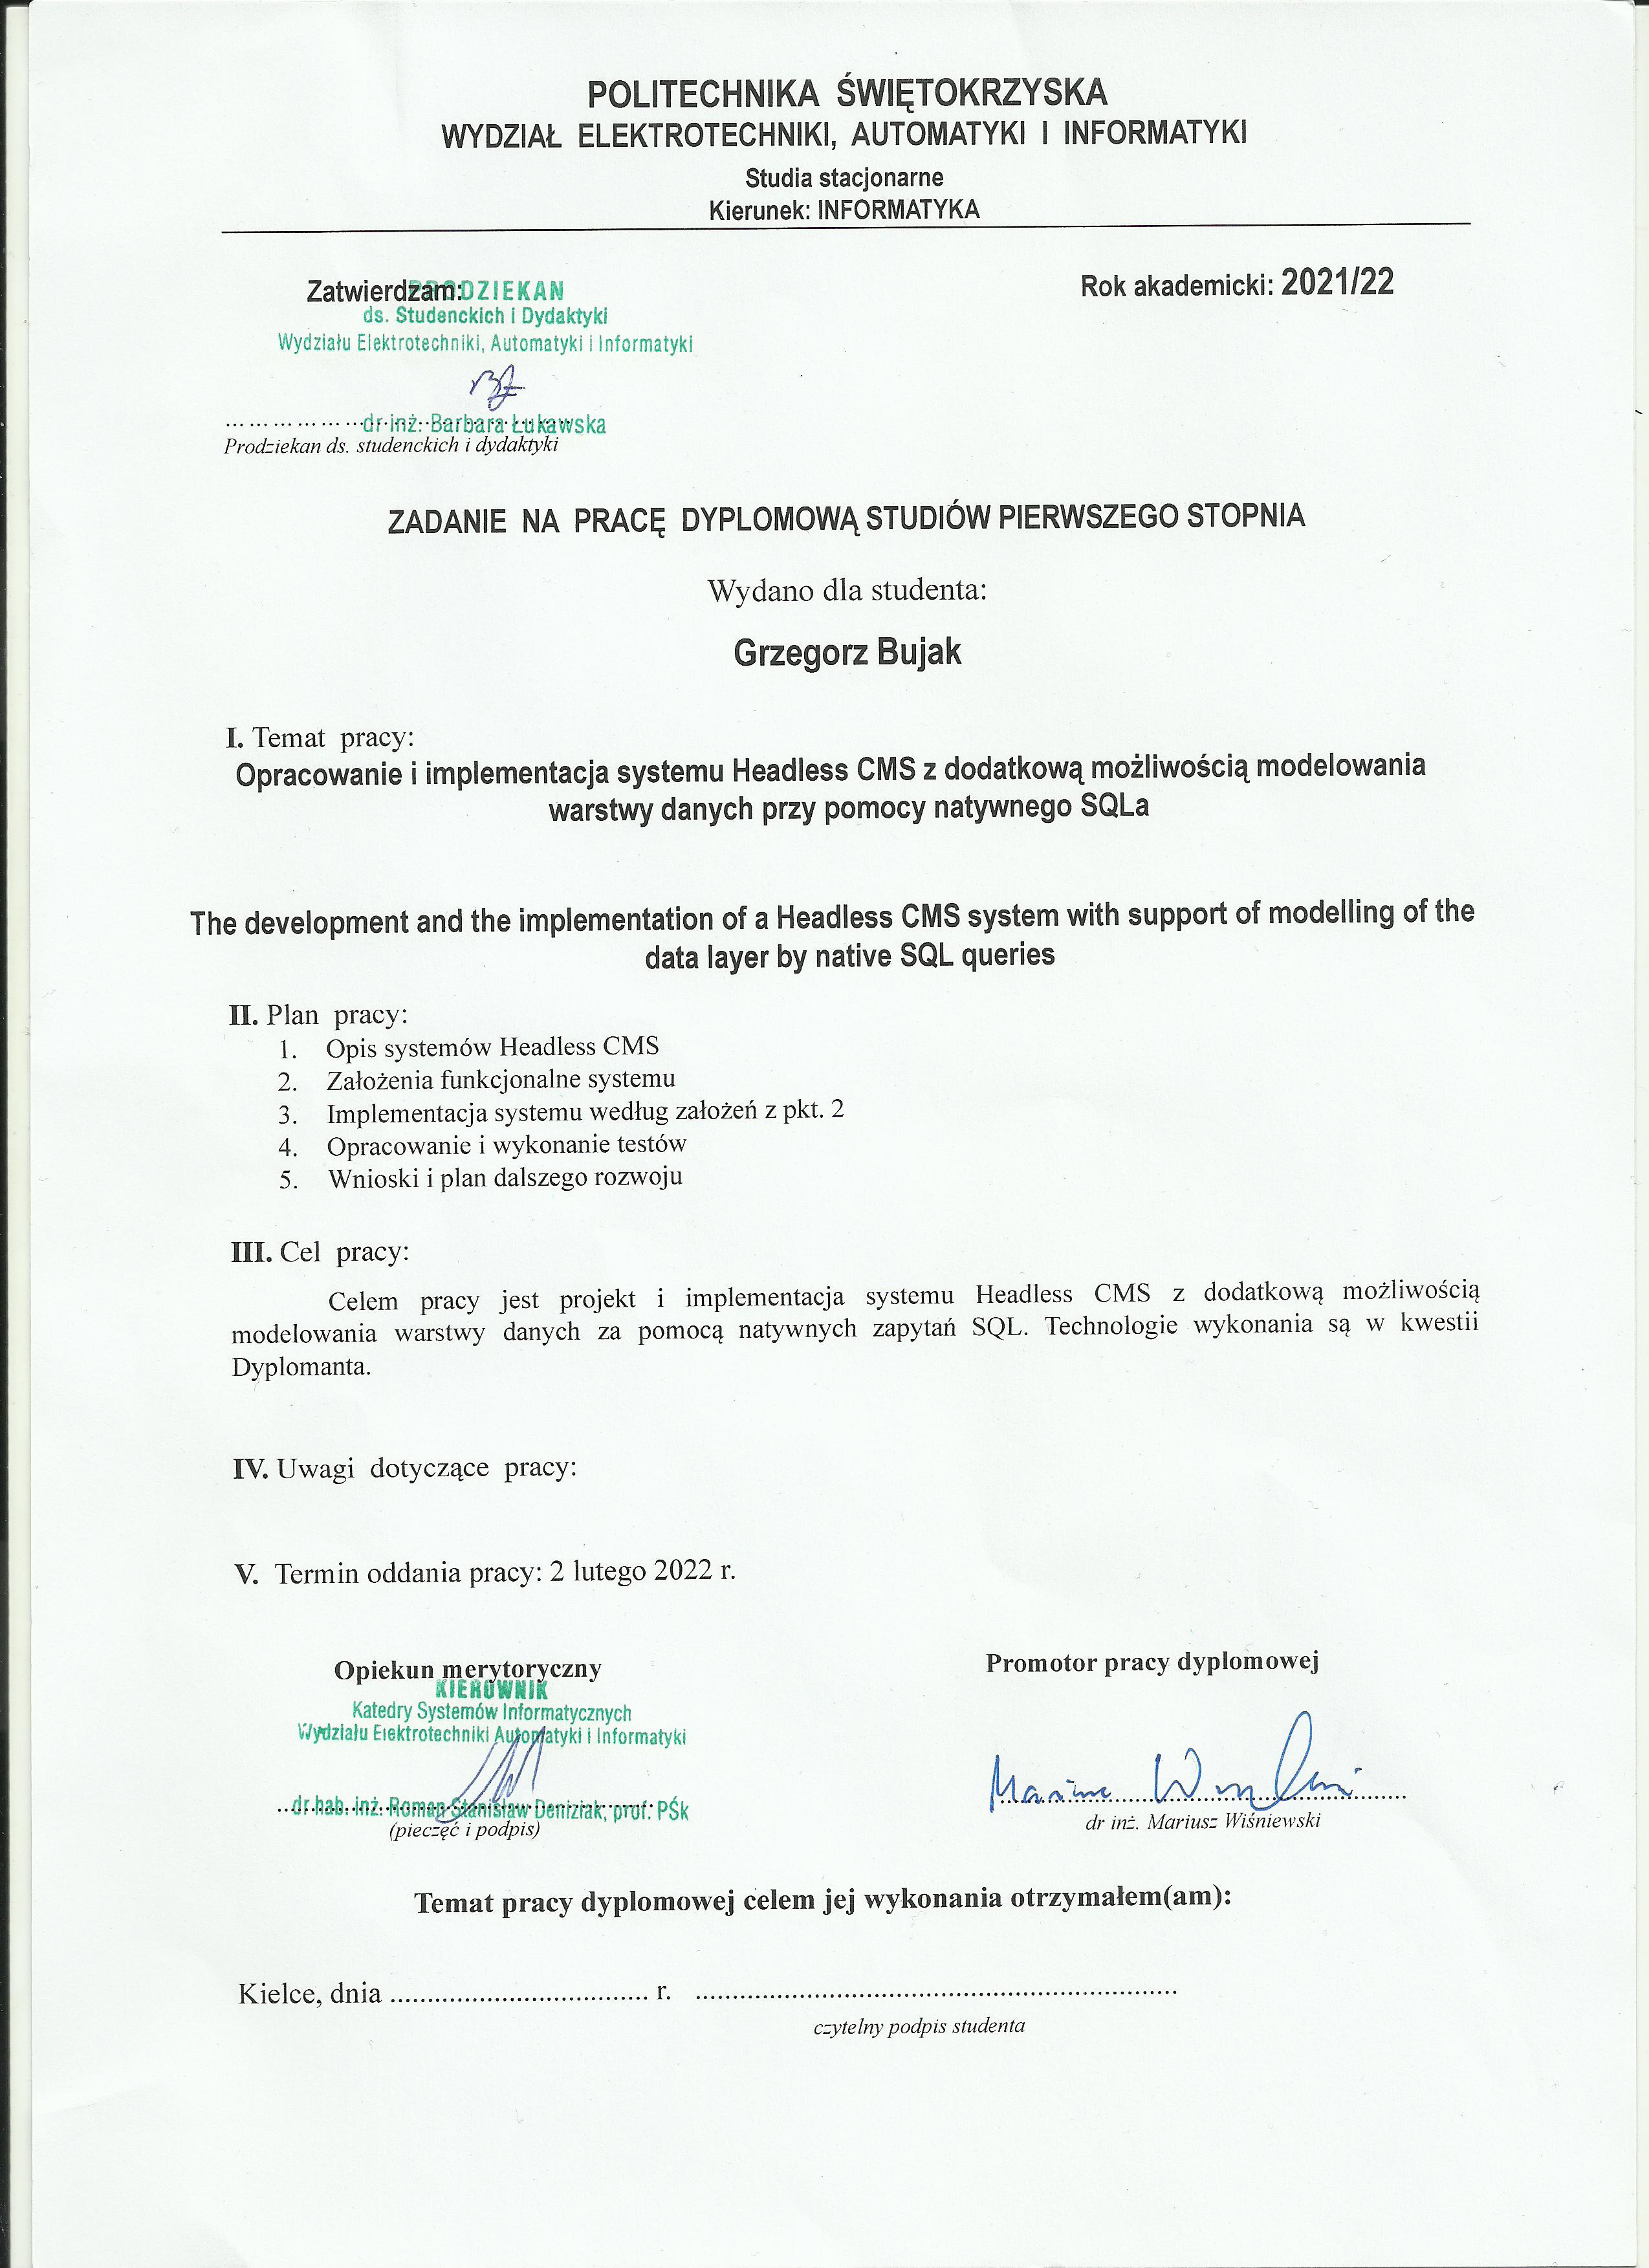
\includegraphics{./img/oryginal.jpg}}
\restoregeometry

%\afterpage{\null\newpage}
\clearpage

\newgeometry{top=0cm}
\centerline{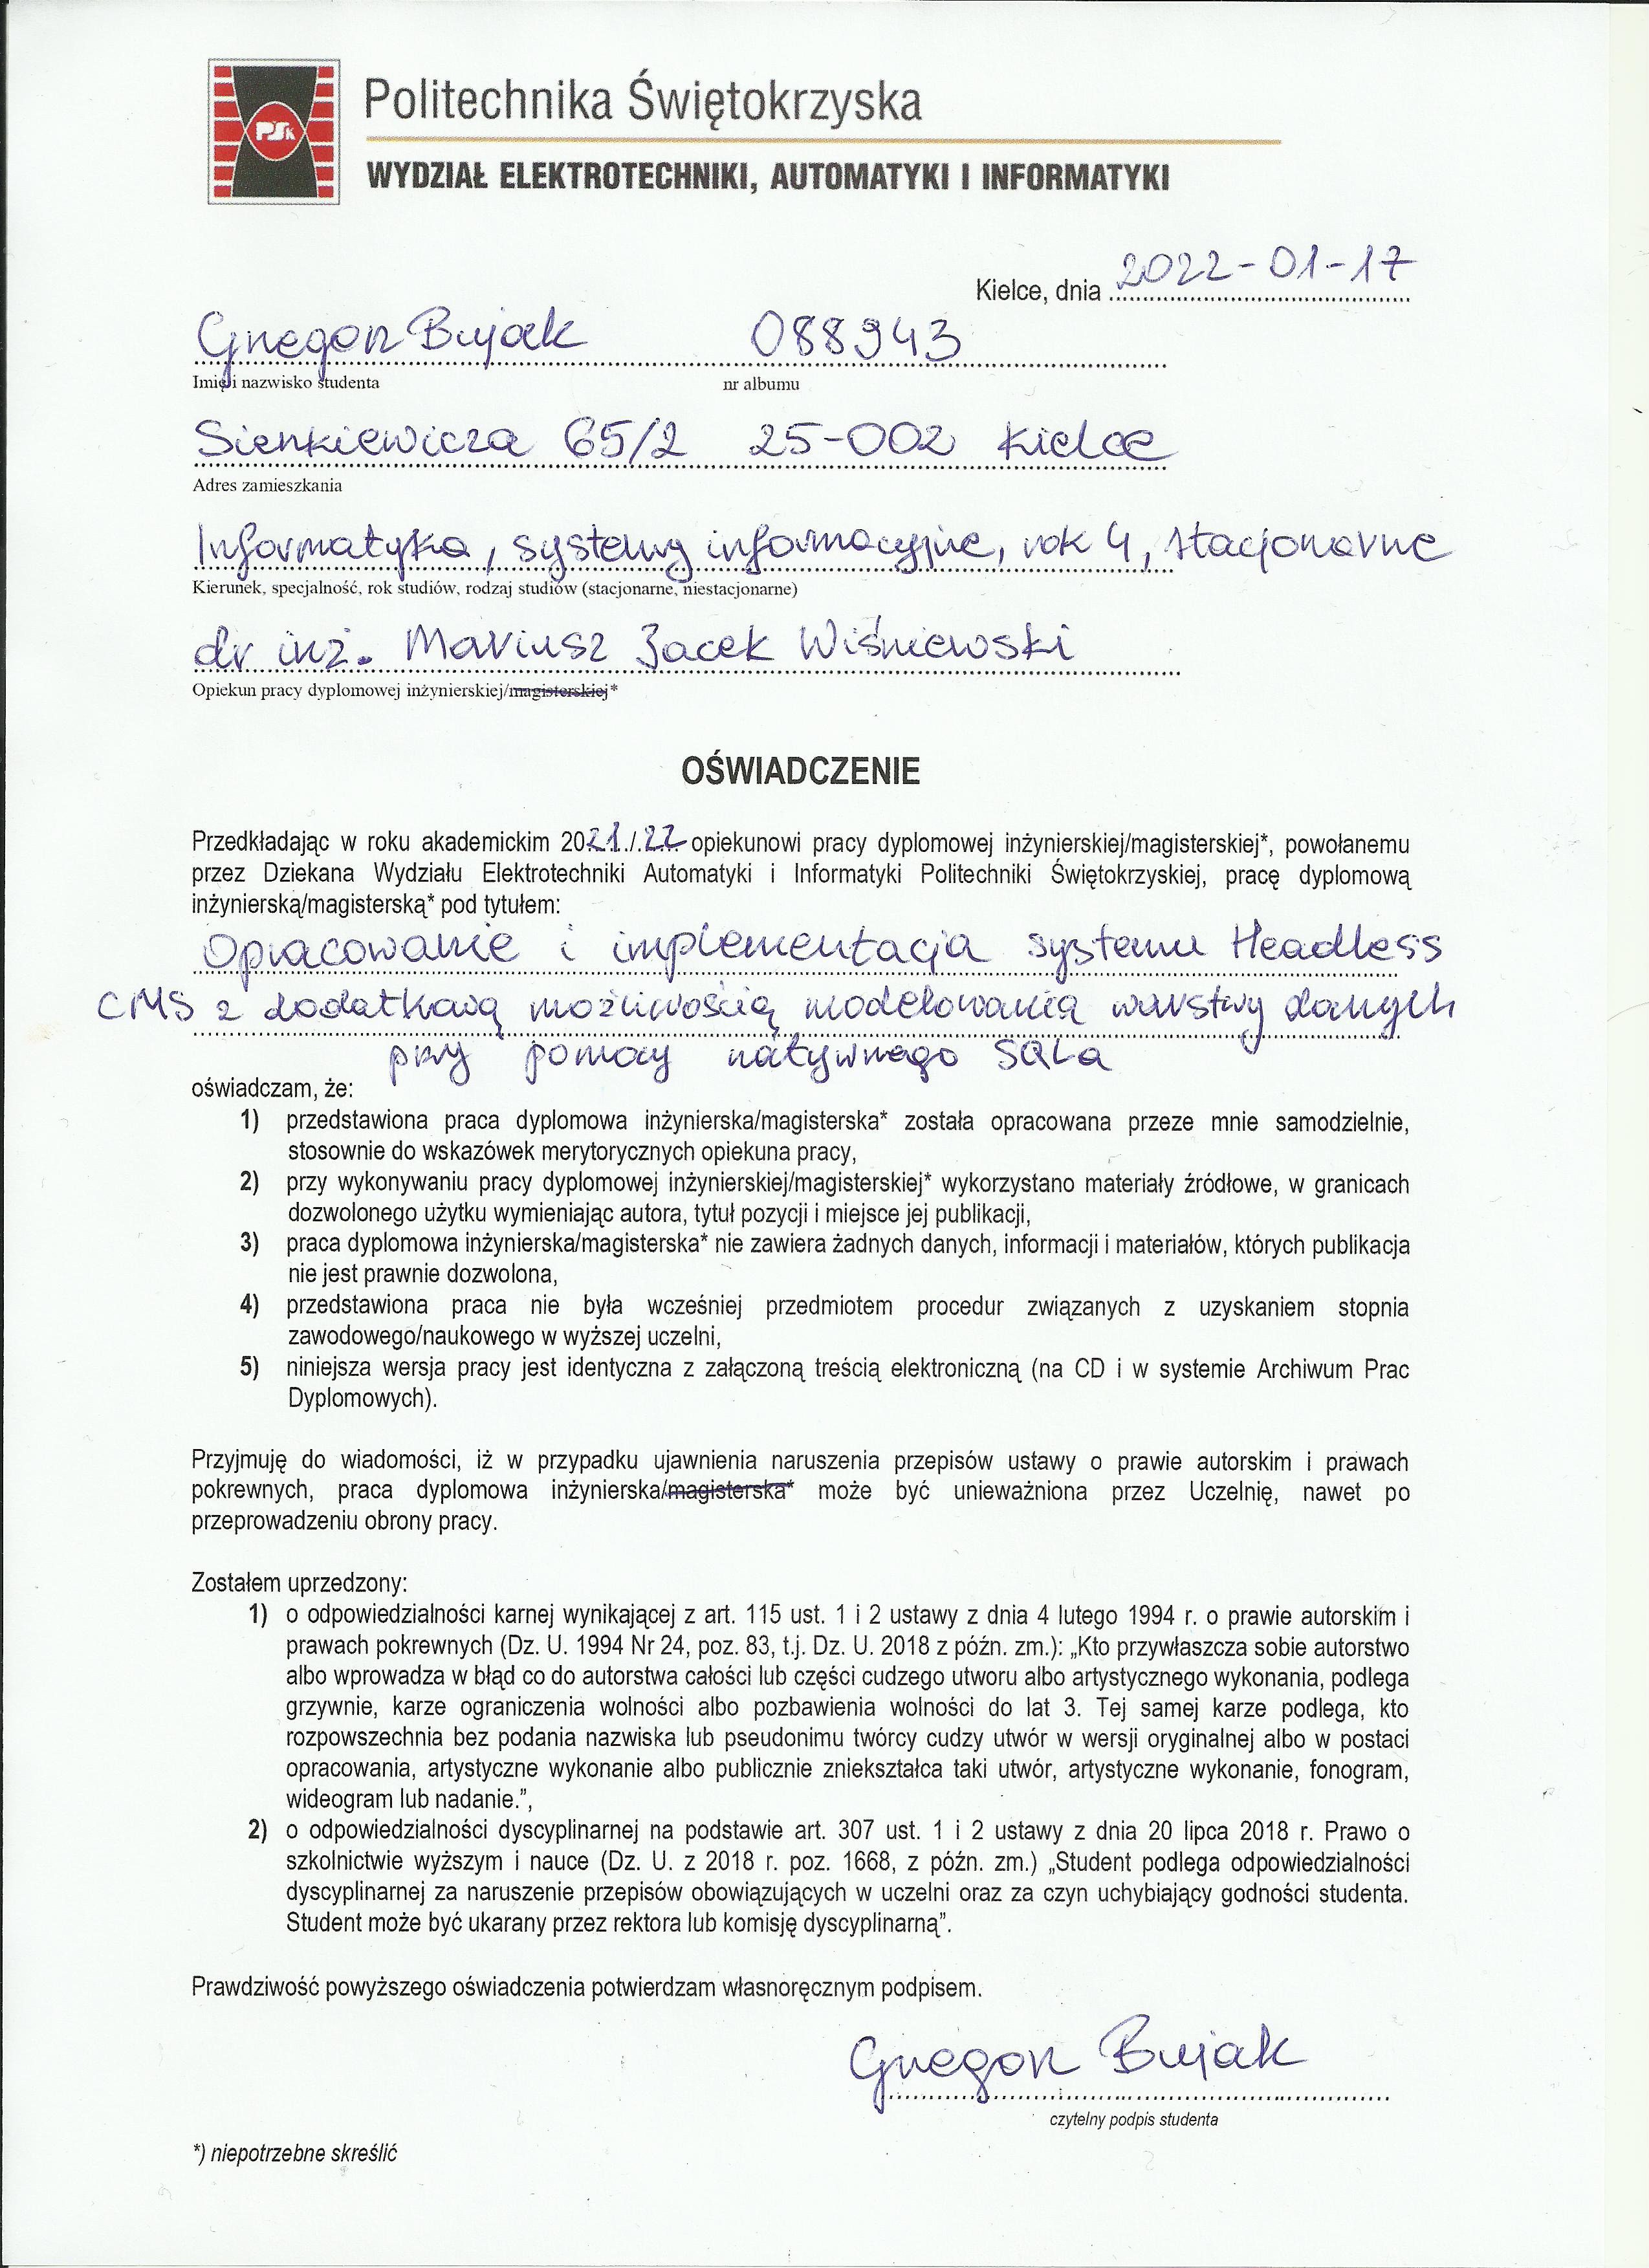
\includegraphics{./img/oswiadczenie.jpg}}
\restoregeometry

\afterpage{\null\newpage}
\clearpage

\begin{center}
    \arialnarrowbold\fontsize{14pt}{14pt}\selectfont\bfseries
    Opracowanie i implementacja systemu Headless CMS z dodatkową możliwością modelowania warstwy
    danych przy pomocy natywnego SQLa
\end{center}

{\arialnarrowbold\fontsize{14pt}{14pt}\selectfont\bfseries \noindent Streszczenie}

\vspace{.5cm}

Systemy CMS oraz Headless CMS mają tendencję do ograniczania możliwości
operowania na danych do statycznych operacji zdefiniowanych przez system. Może
to powodować trudności, gdy wymagane jest wykonanie skomplikowanych operacji na
bazie danych. Ponadto, wysyłanie zapytań do bazy danych, z której korzysta
system CMS jest często odradzanie i niewspierane przez twórców systemu CMS.
Celem pracy dyplomowej jest napisanie systemu Headless CMS, który nie ogranicza
możliwości manipulacji bazą danych. Przygotowany system CMS osiąga ten cel,
przez umożliwienie administratorom wykonywania natywnych zapytań SQL na bazie
danych, z której korzysta system.  Kolejną kluczową funkcją jest pozwolenie
administratorom na definiowanie zapytań, które zostaną wykonane przy zapytaniu
HTTP do systemu CMS, i których dane wynikowe zostaną zwrócone w odpowiedzi HTTP.

\vspace{.5cm}

\noindent Słowa kluczowe: CMS, Headless CMS, bazy danych, SQL, zarządzanie treścią,
warstwa danych

\vspace{1cm}

\begin{center}
    \arialnarrowbold\fontsize{14pt}{14pt}\selectfont\bfseries
    The development and the implementation of a Headless CMS system with support of modelling of the
    data layer by native SQL queries
\end{center}

{\arialnarrowbold\fontsize{14pt}{14pt}\selectfont\bfseries \noindent Summary}

\vspace{.5cm}

CMS and Headless CMS systems have a tendency to limit the ability to operate on
data to static operations defined by the system. It can cause difficulties when
it's necessary to execute complex operations on the database. Furthermore,
sending queries to the database used by the CMS system is often discouraged and
not supported by the authors of the CMS system. The aim of the thesis is to
prepare a Headless CMS system, which does not limit the ability of manipulating
the database. The aim is achieved by allowing the administrators to execute
native SQL queries on the database used by the system. Another key feature is to
let administrators define queries which will be executed after an HTTP request
to the CMS system and the resulting data will be returned in the HTTP response.

\vspace{.5cm}

\noindent Keywords: CMS, Headless CMS, databases, SQL, content management,
data layer

\afterpage{\null\newpage}
\clearpage


\pagenumbering{arabic}
{\arialnarrowbold\tableofcontents}

% \afterpage{\null\newpage}

\clearpage


\section{WSTĘP}

W ostatnich latach można zaobserwować zanikanie podziału pomiędzy mediami
drukowanymi a internetowymi. Większość organizacji publikujących treści prowadzi
strony internetowe. Wiele innych organizacji nie zajmujących się mediami zmaga
się z problemem zarządzania treścią, którą produkują \cite{Mauthe_2004}. 

Programy, które wspomagają tworzenie i zarządzanie treścią nazywa się systemami
zarządzania treścią (ang. content management system — CMS). Do tych aplikacji
zaliczają się dość proste aplikacje służące do zarządzania plikami, jak i
skomplikowane systemy obsługujące wiele rodzajów danych i urządzeń.

Pośród organizacji, które korzystają z systemów zarządzania treścią są między
innymi: CNN, New York Times, Fox News, Wall Street Journal, Armia Stanów
Zjednoczonych. Wszystkie te organizacje korzystają z sytemu Wordpress. Ponadto,
oprócz dużych organizacji, serwis wordpress.com w roku 2009 udostępniał usługi
ponad trzem i pół miliona blogom \cite{brazell2010wordpress}. Mimo to, nie
powstał jeszcze uniwersalny system CMS, który spełniłby zapotrzebowania zarówno
małych instytucji, jak i dużych organizacji, które przechowują duże ilości
danych. Wątpliwe jest nawet, czy taki system mógłby zostać zbudowany, ponieważ
wymagania z różnych przypadków użycia są zupełnie inne \cite{Mauthe_2004}.

Ostatnio, popularne stały się systemy headless CMS \cite{WhyHeadlessCMS}. Są to
systemy CMS pozbawione warstwy prezentacji. Są one zazwyczaj mniej skomplikowane
od tradycyjnych systemów i nie ograniczają wyboru technologii, której można użyć
do implementacji niestandardowej warstwy prezentacji. Systemy te dobrze
spełniają się w architekturze mikroserwisów, lub gdy produkowane treści są
wyświetlane w różnych formach — na przykład na stronie internetowej i w
aplikacji mobilnej \cite{WhyHeadlessCMS}.

\medspace

Zdaniem autora pracy, mimo że systemy headless CMS nie ograniczają warstwy
prezentacji, nie oferują większych, niż tradycyjne systemy możliwości operowania
na warstwie danych. Z tego powodu, w ramach tej pracy, przygotowano system
headless CMS, którego założeniem było nie ograniczanie możliwości operowania na
bazie danych przez umożliwienie administratorom wykonywania natywnych zapytań
SQL.

Kolejnym punktem, gdzie ograniczane są możliwości administratora jest
definiowanie własnych punktów końcowych. Większość systemów CMS zupełnie nie
posiada takiej funkcji, lub wymaga ona pisania przez administratora kodu w
języku innym, niż SQL. Z tego powodu, kolejnym założeniem przygotowanego systemu
było umożliwienie administratorom definiowania własnych punktów końcowych HTTP i
zapytań SQL, które zostaną wykonane przy wywołaniu punktów końcowych i których
wyniki zostaną zwrócone w odpowiedzi HTTP.

\vspace{2cm}

W rozdziale 2 przedstawione zostały systemy CMS jak i inne systemy spełniające
pewien zakres problemów, który chce spełnić przygotowany w ramach pracy system.
W celu uzasadnienia potrzeby przygotowania systemu, zwrócono uwagę na problemy,
które nie są rozwiązane przez poszczególne systemy dostępne na rynku. W
rozdziale 3 przedstawiono założenia projektowe funkcjonalne i niefunkcjonalne
tworzonego systemu. W rozdziale 4 omówiono szczegółowo, jak zaimplementowano
każdą z kluczowych funkcji systemu. W rozdziale 5 omówiono używane przy pisaniu
programu sposoby weryfikacji działania kodu. Pracę kończy rozdział z
podsumowaniem i planem dalszego rozwoju.


\FloatBarrier

\section{CEL I ZAKRES PRACY}

\subsection{Cel pracy}

Celem pracy było przygotowanie systemu CMS. System powinien zawierać większość
funkcji dostępnych w typowym systemie CMS, jak tworzenie nowych typów danych i
manipulacja danymi znajdującymi się w systemie, jednak nie są to główne funkcje
systemu. Głównym założeniem przy projektowaniu i implementacji było stworzenie
sytemu, który nie ogranicza możliwości operowania danymi przez administratora.

Główny cel został osiągnięty przez pozwolenie administratorowi na wykonywanie
natywnych zapytań SQL na bazie danych. Zaimplementowano aplikacje frontend i
backend, które razem umożliwiają administratorowi wygodne pisanie zapytań SQL i
testowanie ich wpływu na bazę danych.

Nie mniej ważnym założeniem było umożliwienie administratorowi definiowania
punktów końcowych, których wywołanie zapytaniem HTTP powoduje wykonanie
zdefiniowanego przez administratora drzewa zapytań SQL. Przygotowany edytor
pozwala na modelowanie struktury danych, które zostaną zwrócone w odpowiedzi
HTTP.

\subsection{Zakres funkcji systemu}

Program przygotowany w ramach pracy można podzielić na dwie części: frontend i
backend:

\begin{enumerate}
    \item Frontend.

    \begin{itemize}

        \item Aplikacja SPA wykorzystującą bibliotekę react.js. Strona
        porozumiewa się z serwerem za pomocą API REST.
        
        \item Jest napisany w języku Typescript i wykorzystuje system typów w
        każdym miejscu, gdzie jest to możliwe.

        \item Strona jest responsywna dzięki zastosowanym nowoczesnym opcjom CSS
        - grid i flexbox. Strona korzysta ze zmiennych CSS. Zmienne CSS
        umożliwiły łatwą implementację funkcji zmiany motywu aplikacji przez
        użytkownika.

        \item Implementuje ważniejsze funkcje typowego panelu administratora
        systemu zarządzania treścią: tworzenie nowych tabel, zarządzanie danymi
        w tabeli.

        \item Implementuje zaawansowany edytor SQL z podświetlaniem składni,
        funkcją zmiany kolejności zapytań, funkcją tymczasowego wyłączania
        zapytania. Wyświetla wyniki każdego zapytania pod kodem zapytania.
        Pozwala pisać zapytanie testowe, którego wynik zostanie pobrany przed
        wykonaniem listy zapytań jak i po wykonaniu. Pozwala na wygenerowanie
        diagramu ER przed i po wykonaniu listy zapytań. Pozwala na testowanie
        listy zapytań z pomocą transakcji, która zostanie wycofana przed zwrotem
        danych.

        \item Implementuje edytor punktów końcowych pozwalający na pisanie
        złożonych drzew zapytań, w których zapytania podrzędne mają dostęp do
        danych wynikających z wykonania zapytań nadrzędnych. Administrator może
        testować punkt końcowy przed wdrożeniem z wykorzystaniem edytora danych
        testowych. Administrator może ograniczać możliwość wywołania punktu
        końcowego do listy grup użytkowników.

        \item Implementuje interfejs tworzenia użytkowników.

    \end{itemize}

    \item Backend.

    \begin{itemize}

        \item Backend aplikacji został napisany w języku rust. Jest
        asynchroniczny, co pozwala na obsługiwanie wielu zapytań na mniejszej
        ilości wątków. Wykorzystuje asynchroniczny runtime Hyper.

        \item Współpracuje z bazą danych PostgreSQL. Używa tabel
        zawierających dane o tabelach w bazie danych, przez co nie musi sam
        przechowywać metadanych o tabelach.

        \item Korzysta z transakcji. Są używane do testowania pisanych
        przez administratora zapytań SQL.

        \item Implementuje generowanie diagramu ER w składni mermaid.js z danych
        pobranych z tabel zawierających metadane o tabelach w bazie danych.

        \item Implementuje bezpieczne wykonywanie drzewa zapytań SQL z użyciem
        niezaufanych danych z przychodzącego zapytania HTTP. Zapytania podrzędne
        mają dostęp do zapytań nadrzędnych. Każde wykorzystanie danych w
        zapytaniach jest zabezpieczone przed atakami SQL injection.

        \item Implementuje system użytkowników z wykorzystaniem technologii json
        web token. Bezpiecznie przechowuje hasła użytkowników za pomocą
        algorytmu Argon2.

    \end{itemize}

\end{enumerate}


\FloatBarrier

\section{PRZEGLĄD ISTNIEJĄCYCH ROZWIĄZAŃ}

\subsection{Wordpress}

Pierwszym omawianym systemem zarządzania treścią jest Wordpress. Jest to
najbardziej popularny CMS. Ten system został napisany z myślą o prezentowaniu
treści w formie strony HTML. Wordpress jest napisany w języku PHP i do działania
wymaga zainstalowania serwera HTTP. Pierwsze wydanie systemu miało miejsce w
roku 2003 i od tamtej pory system jest ciągle rozwijany.

Wordpress pozwala na definiowanie własnych modeli, ale nie jest to wspierane w
domyślnym panelu administratora. Do stworzenia nowego typu danych, wymagane jest
wywołanie funkcji PHP udostępnionej przez Wordpress, do której nie ma domyślnie
interfejsu użytkownika. Polecanym przez twórców sposobem tworzenia nowych typów
danych jest zainstalowanie wtyczki, która implementuje taki interfejs
\cite{WordpressCustomType}.

% https://wordpress.stackexchange.com/questions/158742/add-custom-objects-entities-to-wordpress
% https://developer.wordpress.org/reference/functions/register_post_type/

Pisanie własnych zapytań SQL jest możliwe, ale podobnie jak definiowanie
niestandardowych typów, domyślnie nie posiada interfejsu. W celu napisania
własnego zapytania, trzeba to zrobić z poziomu PHP, lub zainstalować wtyczkę
umożliwiającą pisanie własnych zapytań z panelu administratora.

W wersji 5.0 Wordpress, dodano nowy edytor ``Gutenberg'' pozwalający na
tworzenie postów opartych o bloki. Jest to mniej skomplikowana alternatywa dla
stosowanych do tej pory tzw. ``online rich-text editor''. Edytory blokowe
pozwalają na tworzenie wpisów składających się z bloków. Blok może zawierać
tekst lub media. Bloki tekstowe mogą reprezentować nagłówek lub paragraf, a
paragrafy mogą mieć fragmenty z ograniczonym stylizowaniem jak na przykład
pogrubieniem czcionki. Wpisy w formie bloków są łatwiejsze w przechowywaniu i
wyświetlaniu na stronie HTML. Nie jest konieczne na przykład parsowanie treści
wpisów, żeby wydobyć informacje o zdjęciach, jakie zostały zamieszczone we
wpisie.

Wpisy oparte o bloki mogą być wygodnie tworzone w dużo prostszych edytorach.
Zmniejsza to potrzebę stosowania skomplikowanych systemów CMS do zarządzania
treścią.

Podsumowując, Wordpress to oprogramowanie, które dobrze spełnia potrzeby autora
bloga. Znaczną zaletą systemu Wordpress jest ekosystem wtyczek pozwalających na
rozwiązanie większości problemów związanych z zarządzaniem danymi.

System Wordpress domyślnie znacznie ogranicza możliwości administratora. W celu
wykonywania niestandardowych operacji na bazie danych, administrator musi
polegać na wtyczkach, lub samemu napisać umożliwiające to wtyczki. Zwiększa to
znacznie wymagania wiedzy wobec administratora.

Pomimo tego, możliwe jest skonfigurowanie systemu Wordpress w taki sposób, żeby
spełniał wszystkie funkcje przygotowanego w ramach tej pracy systemu. Taka
konfiguracja byłaby jednak mniej stabilna od sytemu, który powstawał w celu
spełnienia tych celów. Niezbędne byłoby poleganie na dużej ilości wtyczek, lub
napisanie tych wtyczek samemu, co może być bardziej skomplikowane, niż napisanie
systemu backend spełniającego potrzeby jednej strony internetowej.

(TODO: cite Wordpress bible)

\subsection{Strapi}

Strapi to sytem Headless CMS. Nie posiada on interfejsu użytkownika. Dane
wprowadzane do systemu są pobierane za pomocą API REST. Domyślne API ma
ograniczoną funkcjonalność. Pobieranie danych z CMS jest ograniczone do
pobierania wszystkich wpisów danego typu, lub jednego wpisu, ale tylko po id.

Strapi umożliwia tworznie własnych punktów końcowych. Administrator może ustawić
ścieżkę i funkcję, która obsłuży zapytania na daną ścieżkę. Nie da się jednak
zrobić tego w panelu administratora. Administrator chcąc stworzyć niestandardowy
punkt końcowy musi sam napisać funkcje, które obsłużą zapytania w języku
JavaScript. Jest to porównywalnie skomplikowane do napisania kontrolera w
zwykłej aplikacji internetowej. Ponadto, na administratora są nałożone pewne
ograniczenia. System Strapi wspiera wiele baz danych, w tym MongoDB, która nie
wspiera SQL. Z tego powodu, nie jest możliwe pisanie natywnych zapytań do bazy
danych. Do operacji na bazie danych Strapi udostępnia ``query engine''. Jest to
biblioteka do operacji na bazie danych z poziomu języka JavaScript. API
udostępnione programistom przez ``query engine'' jest znacznie ograniczone w
porównaniu do natywnego SQL. Nie można używać funkcji specyficznych do wybranej
bazy danych. Operacje są ograniczone do prostych zapytań CRUD.

Strapi umożliwia operowanie na danych za pomocą GraphQL. Ta opcja pozwala na
pobieranie konkretnych danych o wpisie zamiast całości informacji. W celu
pobierania niestandardowych informacji, wymagane jest pisanie własnych
``resolwerów''. Pisanie resolwerów przypomina pisanie funkcji obsługującej
zapytania do REST API. Wymaga pisania kodu źródłowego w języku JavaScript.

Podsumowując, Strapi jest dobrym wyborem, jeśli potrzebny jest system CMS
pozwalający na bardziej złożone od CRUD operacje na danych. Niezbędne będzie
jednak pisanie własnych funkcji obsługujących zapytania z wykorzystaniem
ograniczonego API do operacji na bazie danych.

Znacznym minusem Strapi są duże wymagania wobec sprzętu. Minimalna ilość pamięci
to 2GB \cite{StrapiDeployment}. Nie jest to problem dla przedsiębiorstw, ale
może to zwiększyć koszty osób zarządzających mniejszymi stronami internetowymi.

% https://docs.strapi.io/developer-docs/latest/setup-deployment-guides/deployment.html

\subsection{PostgREST}

PostgREST nie jest systemem CMS. Twórcy definiują ten program, jako samodzielny
serwer internetowy, który przemienia bazę danych Postgres w API REST
\cite{PostgrestDefinition}. Mimo tego, PostgREST spełnia dużą część założeń tej
pracy dyplomowej.

PostgREST jest przeznaczony do pracy tylko z bazą danych PostgreSQL. Dzięki
takiej specjalizacji, umożliwia on korzystanie z funkcji specyficznych dla bazy
danych PostgreSQL. Umożliwia wyłuskiwanie danych z kolumn o typie \texttt{json}
\cite{PostgrestJson} i korzystanie z funkcji full-text search \cite{PostgrestFts}.

Minusem serwera PostgREST jest to, że zapytania SQL są kodowane w parametrach
zapytania HTTP, co zmniejsza czytelność zapytań SQL. Można to zauważyć w
przykładowym zapytaniu z dokumentacji PostgREST pobierającym dane z wielu tabel:

\begin{verbatim}
GET /films?select=title,actors!inner(first_name,last_name)
        &actors.first_name=eq.Jehanne HTTP/1.1
\end{verbatim}

\noindent Powinno zwrócić dane JSON:

\begin{verbatim}
[{
    "title": "The Haunted Castle",
    "actors": [{
        "first_name": "Jehanne",
        "last_name": "d'Alcy"
    }]
}]
\end{verbatim}

Podsumowując, jeśli aplikacja będzie wymagała dużej ilości niestandardowych
operacji na bazie danych, PostgREST z dodatkiem prostej aplikacji serwerowej
jest dobrym wyborem, jeśli nie potrzeba panelu administratora. Jest to jedyne
omawiane do tej pory narzędzie, które nie ogranicza w większym stopniu
możliwości operowania na bazie danych.

\subsection{Podsumowanie}

Podsumowując, można zauważyć, że na rynku nie ma popularnego narzędzia
spełniającego założenia pracy. Istnieje wiele narzędzi, które można dostosować
do założeń pracy, ale takie zastosowanie nie jest zamierzone przez twórców, lub
wymaga pisania kodu poza zapytaniami SQL.


\FloatBarrier

\section{PROJEKT SYSTEMU}

\subsection{Aplikacje wchodzące w skład systemu}

Program przygotowany w ramach pracy można podzielić na dwie części: frontend i
backend:

\begin{enumerate}
    \item Frontend.

    \begin{itemize}

        \item Aplikacja SPA wykorzystującą bibliotekę react.js. Strona
        porozumiewa się z serwerem za pomocą API REST.
        
        \item Jest napisany w języku Typescript i wykorzystuje system typów w
        każdym miejscu, gdzie jest to możliwe.

        \item Strona jest responsywna dzięki zastosowanym nowoczesnym opcjom CSS
        - grid i flexbox. Strona korzysta ze zmiennych CSS. Zmienne CSS
        umożliwiły łatwą implementację funkcji zmiany motywu aplikacji przez
        użytkownika.

        \item Implementuje ważniejsze funkcje typowego panelu administratora
        systemu zarządzania treścią: tworzenie nowych tabel, zarządzanie danymi
        w tabeli.

        \item Implementuje zaawansowany edytor SQL z podświetlaniem składni,
        funkcją zmiany kolejności zapytań, funkcją tymczasowego wyłączania
        zapytania. Wyświetla wyniki każdego zapytania pod kodem zapytania.
        Pozwala pisać zapytanie testowe, którego wynik zostanie pobrany przed
        wykonaniem listy zapytań jak i po wykonaniu. Pozwala na wygenerowanie
        diagramu ER przed i po wykonaniu listy zapytań. Pozwala na testowanie
        listy zapytań z pomocą transakcji, która zostanie wycofana przed zwrotem
        danych.

        \item Implementuje edytor punktów końcowych pozwalający na pisanie
        złożonych drzew zapytań, w których zapytania podrzędne mają dostęp do
        danych wynikających z wykonania zapytań nadrzędnych. Administrator może
        testować punkt końcowy przed wdrożeniem z wykorzystaniem edytora danych
        testowych.

        \item Implementuje interfejs tworzenia użytkowników.

    \end{itemize}

    \item Backend.

    \begin{itemize}

        \item Backend aplikacji został napisany w języku rust. Jest
        asynchroniczny, co pozwala na obsługiwanie wielu zapytań na mniejszej
        ilości wątków. Wykorzystuje asynchroniczny runtime Hyper.

        \item Współpracuje z bazą danych PostgreSQL. Używa tabel
        zawierających dane o tabelach w bazie danych, przez co nie musi sam
        przechowywać metadanych o tabelach.

        \item Korzysta z transakcji. Są używane do testowania pisanych
        przez administratora zapytań SQL.

        \item Implementuje generowanie diagramu ER w składni mermaid.js z danych
        pobranych z tabel zawierających metadane o tabelach w bazie danych.

        \item Implementuje bezpieczne wykonywanie drzewa zapytań SQL z użyciem
        niezaufanych danych z przychodzącego zapytania HTTP. Zapytania podrzędne
        mają dostęp do zapytań nadrzędnych. Każde wykorzystanie danych w
        zapytaniach jest zabezpieczone przed atakami SQL injection.

        \item Implementuje system użytkowników z wykorzystaniem technologii json
        web token. Bezpiecznie przechowuje hasła użytkowników za pomocą
        algorytmu Argon2.

    \end{itemize}

\end{enumerate}

\subsection{Projekt aplikacji frontend}




\FloatBarrier

\section{IMPLEMENTACJA KLUCZOWYCH FUNKCJI}

\subsection{Tworzenie nowych typów danych}

Funkcjonalność tworzenia nowych typów danych nie wyróżnia przygotowanego systemu
od systemów CMS dostępnych na rynku. Jest zaimplementowana, jako lista
formularzy. Każdy formularz odpowiada jednej kolumnie w nowo utworzonej tabeli.
Administrator może dodawać nowy formularz, lub kasować już istniejący.

Pojedyńczy formularz zawiera następujące elementy:

\begin{itemize}

    \item Pole tekstowe, gdzie administrator podaje nazwę kolumny.

    \item Menu rozwijane pozwalające na wybór typu kolumny.

    \item Pole wyboru, które pozwala określić administratorowi, czy kolumna może
    zawierać wartości \verb|null|.

    \item Pole wyboru, które pozwala określić czy kolumna posiada wartość
    domyślną wraz z polem tekstowym, które pojawia się, gdy administrator
    oznaczy kolumnę jako posiadającą wartość domyślną, gdzie należy podać
    wartość domyślną.

\end{itemize}

Interfejs tworzenia nowych typów danych jest pokazany na rysunku \ref{tableCreationFigure}.

\begin{figure}[h]
    \centering
    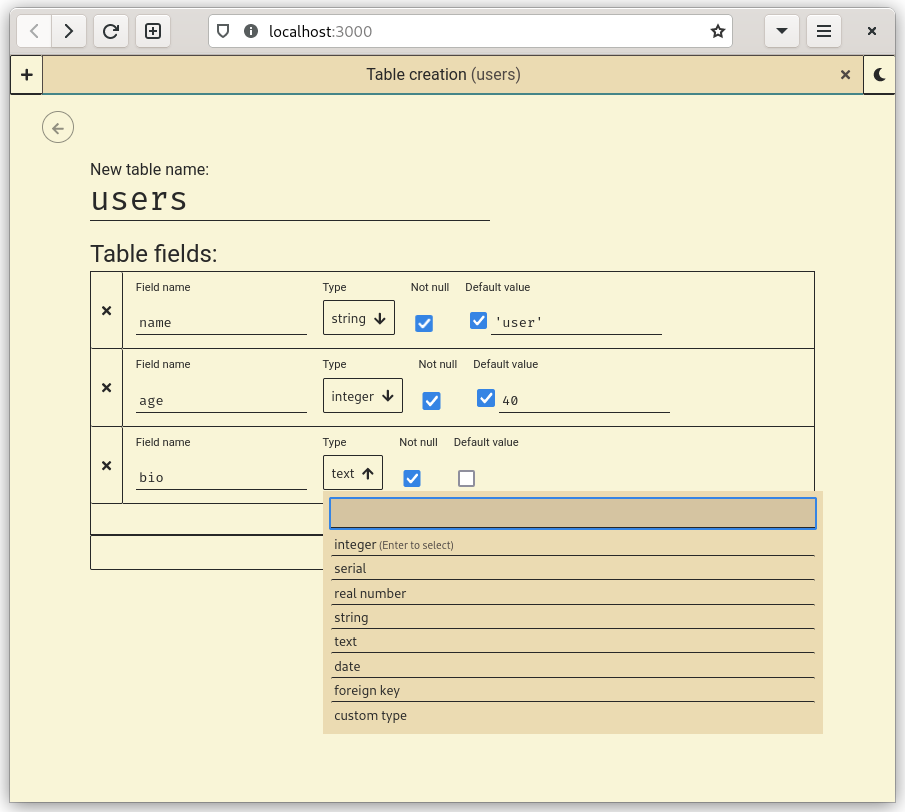
\includegraphics[width=0.8\textwidth]{./img/table_creation.png}
    \caption{Interfejs tworzenia nowego typu danych}
    \label{tableCreationFigure}
\end{figure}

\subsection{Zarządzanie danymi}



\clearpage
\section{WERYFIKACJA PRACY PROGRAMU}
\label{testSection}

\subsection{Testy jednostkowe}

Działanie wszystkich funkcji wchodzących w skład bardziej skomplikowanej logiki
biznesowej programu, zawartej w module \verb|algorithms| zostało zweryfikowane
testami jednostkowymi. Wynik wykonania testów jednostkowych można zobaczyć na
listingu \ref{cargoTestListing}.

\lstinputlisting[
    float=h!,
    basicstyle=\ttfamily\small,
    frame=tb,
    label={cargoTestListing},
    caption={Wykonanie testów jednostkowych}
]{./code/cargoTest.txt}

Działanie testów jednostkowych można opisać następująco:

\begin{itemize}

    \item \verb|mermaid_diagram_generation::tests::works| - test sprawdza
        poprawność działania algorytmu generującego diagram ER w składni
        \verb|mermaid.js|. Do implementacji podawana jest przykładowa struktura
        tabel. Sprawdzane jest, czy wygenerowany diagram jest poprawny.

    \item \verb|sql_variable_parser::tests::parsing_test| - test sprawdza
        podstawową funkcję parsującą SQL wykorzystywaną do implementacji
        bardziej skomplikowanej funkcjonalności parsera.

    \item \verb|sql_variable_parser::tests::parsing_multiple| - test sprawdza
        poprawne działanie parsera SQL, gdy w jednym zapytaniu znajduje się
        większa ilość odwołań do zmiennych.

    \item \verb|sql_variable_parser::tests::bind_vec| - test sprawdza poprawność
        działania funkcji, która przekształca tablicę mieszającą zawierającą
        dostępne zmienne i sparsowany SQL na tablicę wartości, które powinny
        zostać wysłane do bazy danych.

    \item \verb|sql_variable_parser::tests::parsing_endpoint_info| - test
        sprawdza poprawność funkcji parsującej strukturę danych, którą należy
        wysłać do serwera w celu stworzenia nowego punktu końcowego.

    \item \verb|sql_variable_parser::tests::not_closed_panics| - test sprawdza,
        czy program zwraca błąd, gdy do funkcji parsującej SQL podane zostanie
        zapytanie z niepoprawną składnią (niedomknięta klamra).

    \item \verb|endpoint_execution::test::it_works| - test sprawdza podstawowe
        działanie modułu wykonującego drzewo zapytań SQL. Do implementacji
        podawane jest drzewo zkładające się z jednego liścia. Sprawdzane jest,
        czy zapytanie umieszczone w liściu zostało wykonane.
        
    \item \verb|endpoint_execution::test::request_variables_work| - test
        sprawdza poprawne działanie, gdy drzewo zapytań SQL zawiera zapytanie z
        odniesieniem do zmiennej pochodzącej z zapytania HTTP. Sprawdzane jest,
        czy do bazy danych wysyłane jest poprawne zapytanie SQL i poprawne
        zmienne.

    \item \verb|endpoint_execution::test::super_variables_work| - test sprawdza
        poprawne działanie, gdy drzewo zapytań SQL zawiera zapytanie z
        odniesieniem do zmiennej pochodzącej z zapytania nadrzędnego. Do modułu
        podawane jest drzewo z dwoma węzłami. Węzeł podrzędny odnosi się do
        zmiennej będącej wynikiem wykonania węzła nadrzędnego. Sprawdzana jest
        poprawna kolejność wysyłanych zapytań SQL oraz poprawność danych
        wysyłanych razem z zapytaniem podrzędnym.

    \item \verb|endpoint_execution::test::error_when_cant_find_req_variable| -
        test sprawdza, czy program zwróci błąd, gdy zapytanie odnosi się do
        zmiennej wysyłanej z zapytaniem HTTP, która nie istnieje.

    \item \verb|endpoint_execution::test::error_when_cant_find_super_variable| -
        test sprawdza czy program zwróci błąd, kiedy węzeł podrzędny zawiera
        odniesienie do zmiennej z węzła nadrzędnego, która nie istnieje.

    \item \verb|endpoint_execution::test::error_when_too_many_supers| - test
        sprawdza czy program zwróci błąd, gdy zmienna zawarta w drzewie zapytań
        sql odnosi się do zmiennej, która nie może istnieć, bo nazwa zmiennej
        zawiera więcej prefiksów ``\verb|super.|'', niż istnieje węzłów
        nadrzędnych. Do modułu podawane jest drzewo z dwoma węzłami. Węzeł
        podrzędny odnosi się do zmiennej z dwoma prefiksami ``\verb|super.|'',
        ale ma tylko jeden węzeł nadrzędny.

\end{itemize}

\subsection{Testy integracyjne}

Testy integracyjne zostały napisane w programie Postman. Jest to program służący
do testowania API. Testy napisane w tym programie można wyeksportować do pliku
json, który można wykonać z poziomu powłoki tekstowej za pomocą programu
newman. Pozwala to na automatyczne wykonywanie testów.

Wykonanie testów integracyjnych widać na listingu \ref{postmanTestExec}.

% \lstinputlisting[
%     frame=tb,
%     label={postmanTestExec},
%     caption={Wykonanie testów integracyjnych za pomocą programu \verb|newman|.
%         Dla poprawienia przejrzystości usunięto tokeny JWT.}
% ]{./code/newmanIntegration.txt}


\FloatBarrier

Wykonanie testów integracyjnych powinno odbywać się po uruchomieniu aplikacji
backend po raz pierwszy z pustą bazą danych. Stan aplikacji zostaje zachowany
podczas całego działania testów integracyjnych. Działanie to można opisać
następująco:

\begin{enumerate}

    \item Login admin - test sprawdza, czy możliwe jest poprawne zalogowanie do
        konta administratora. Token administratora jest zapisywany i korzystają
        z niego pozostałe testy.

    \item Create users - test wysyła do serwera polecenie stworzenia
        użytkowników, sprawdza czy odpowiedź jest poprawna.

    \item Create table form - test wysyła do serwera polecenie stworzenia
        tabeli. Polecenie nie zawiera zapytania SQL. Jest to wariant polecenia,
        który wysyła aplikacja frontend przy tworzeniu nowego typu danych za
        pomocą formularza.

    \item Get table info - test wysyła do serwera zapytanie o informacje o
        tabelach zawartych w bazie danych. Test sprawdza, czy odpowiedź zawiera
        dane o tabeli stworzonej w teście 3.

    \item Insert data - test wysyła do serwera polecenie dodania danych do
        tabeli. Jest to wariant polecenia, jakie wysyła aplikacja frontend przy
        dodawaniu danych za pomocą formularza.

    \item Get data - test wysyła do serwera zapytanie o informacje zawarte w
        tabeli stworzonej w teście 3. Jest to wariant zapytania, jakie wysyła
        aplikacja frontend w edytorze danych opartym o formularze. Test
        sprawdza, czy dane są takie same, jak te dodane do tabeli w teście 5.

    \item Execute query - test wysyła do serwera zapytanie HTTP z zapytaniami
        SQL. Test wysyła zapytanie tworzące nowe dane w tabeli stworzonej w
        teście 3 oraz zwracające stworzone dane. Zapytanie zostało umieszczone
        poniżej.

        \begin{verbatim}
insert into test_table_one (name, age)
    values ('Adam Nowak', 42)
    returning name, age::text
        \end{verbatim}

        Ponadto, zapytanie zawiera zapytanie SQL wykonywane przed i po wykonaniu
        drzewa zapytań. Jest to zapytanie pobierające wartości z kolumny
        \verb|name| z tabeli \verb|test_table_one|. Test sprawdza czy zapytanie
        zostało poprawnie wykonane oraz czy wartości zapytania wykonywanego
        przed i po drzewie zapytań są poprawne.

    \item Test endpoint - test wysyła do serwera zapytanie będące wariantem
        zapytania, jakie wysyła aplikacja frontend w celu przetestowania
        tworzonego punktu końcowego. Test sprawdza poprawność odesłanej przez
        serwer odpowiedzi.

    \item Create endpoint - test wysyła do serwera zapytanie będące wariantem
        zapytania, które aplikacja frontend wysyła w celu stworzenia punktu
        końcowego. Test spradza, czy odpowiedź od serwera ma kod HTTP 200 OK.

    \item Call endpoint as admin - test wywołuje punkt końcowy stworzony w
        teście 8. Test sprawdza, czy wysłana przez serwer odpowiedź zawiera
        poprawne dane. Test sprawdza, czy administrator może wywoływać dowolne
        punkty końcowe nawet, gdy nie ma go na liście użytkowników, którzy mają
        dostęp do punktu końcowego.

    \item Get endpoints - test wysyła do serwera zapytanie będące wariantem
        zapytania wysyłanego przez aplikację frontend w celu pobrania od serwera
        informacji o istniejących punktach końcowych. Test sprawdza, czy w
        odpowiedzi znajdują się dane o punkcie końcowym stworzonym w teście 8.

    \item Create manager user - test tworzy użytkownika należącego do grupy
        \verb|MANAGERS|. Ta grupa ma dostęp do punktu końcowego stworzonego w
        teście 8.

    \item Try call worker - test próbuje wywołać punkt końcowy przy pomocy konta
        użytkownika stworzonego w teście 2. Użytkownik nie ma uprawnień do
        wywoływania tego punktu końcowego. Test sprawdza, czy zwrócono kod HTTP
        401 oznaczający brak dostępu.

    \item Call manager - test wywołuje punkt końcowy stworzony w teście 8 przy
        użyciu konta kierownika stworzonego w teście 11. Użytkownik ma możliwość
        wywoływania punktu końcowego. Test sprawdza, czy punkt końcowy został
        wywołany.

\end{enumerate}

\subsection{Testy manualne}

Poprawne działanie najważniejszych funkcji aplikacji frontend zostało
zweryfikowane za pomocą testów manualnych. Scenariusze testów manualnych zostały
przedstawione poniżej.

\begin{enumerate}

    \item \textbf{Testowanie poprawnego działania systemu kart.}

        \begin{enumerate}

            \item \textbf{Testowanie poprawnego tworzenia nowej karty.}

                \textbf{Przebieg testu:}

                \begin{enumerate}

                    \item Wciśnięcie przycisku ``+'' po lewej stronie paska
                        kart.

                \end{enumerate}

                \textbf{Spodziewany wynik:}

                Jeśli ostatnia karta znajduje się na widoku startowym, powinna
                zostać wybrana jako aktywna. Jeśli już była aktywna, powinna
                pozostać aktywna.

                Jeśli ostatnia karta nie znajduje się na widoku startowym,
                powinna zostać stworzona nowa karta znajdująca się na widoku
                startowym. Nowa karta powinna zostać wybrana jako aktywna.

            \item \textbf{Testowanie poprawnego zamykania karty.}

                \textbf{Przebieg testu:}

                \begin{enumerate}

                    \item Wciśnięcie przycisku ``x'' po prawej stronie karty,
                        lub wciśnięcie dowolnego miejsca karty środkowym
                        przyciskiem myszki.

                \end{enumerate}

                \textbf{Spodziewany wynik:}

                Jeśli karta, którą spróbowano zamknąć jest jedyną kartą i nie
                jest na widoku startowym, nie powinno się nic stać. Jeśli karta
                jest jedyną i nie jest na widoku startowym, w karcie powinien
                zostać otworzony widok startowy.

                Jeśli karta, którą spróbowano zamknąć nie jest jedyną kartą,
                karta powinna przestać istnieć. Dowolna sąsiedna karta do karty
                zamkniętej powinna zostać wybrana jako aktywna.

            \item \textbf{Testowanie poprawnego zachowania stanu w karcie.}

                \textbf{Przebieg testu:}

                \begin{enumerate}

                    \item Otworzenie w dowolnej karcie komponentu zawierającego
                        stan (na przykład pole tekstowe).

                    \item Zmiana stanu komponentu (na przykład wpisanie dowonego
                        tekstu do pola tekstowego).

                    \item Przełączenie aktywnej karty na dowolną inną kartę.

                    \item Przełączenie aktywnej karty na kartę otwartą w kroku
                        i.

                \end{enumerate}

                \textbf{Spodziewany wynik:}

                Stan komponentu po ponownym otwarciu karty powinien być
                identyczny do stanu przed pierwszym przełączeniem aktywnej
                karty.

        \end{enumerate}

    \item \textbf{Testowanie poprawnego działania edytora zapytań SQL
        wykonywanych natychmiast.}

        \begin{enumerate}

            \item \textbf{Testowanie poprawnego tworzenia nowego zapytania.}

                \textbf{Przebieg testu:}

                \begin{enumerate}

                    \item Wciśnięcie przycisku ``New block'' pod ostatnim
                        polem tekstowym z zapytaniem SQL.

                \end{enumerate}

                \textbf{Spodziewany wynik:}

                Pod ostatnim edytorem zapytania SQL pojawi się nowy edytor
                zapytania SQL.


            \item \textbf{Testowanie poprawnego usuwania zapytania SQL.}

                \textbf{Przebieg testu:}

                \begin{enumerate}

                    \item Wciśnięcie przycisku ``Delete'' po lewej stronie pola
                        teskstowego z zapytaniem SQL.

                \end{enumerate}

                \textbf{Spodziewany wynik:}

                Jeśli edytor jest jedynym edytorem, treść zapytania SQL zostanie
                usunięta.

                Jeśli edytor nie jest jedynym edytorem, zostanie usunięty z
                listy edytorów.

            \item \textbf{Testowanie poprawnego wyłączania zapytania SQL.}

                \textbf{Przebieg testu:}

                \begin{enumerate}

                    \item Wciśnięcie przycisku ``Disable'' po lewej stronie pola
                        teskstowego z zapytaniem SQL.

                    \item Wciśnięcie przycisku ``Enable'' po lewej stronie pola
                        teskstowego z zapytaniem SQL.

                \end{enumerate}

                \textbf{Spodziewany wynik:}

                Po wciśnięciu przycisku ``Disable'', tło zostanie przyciemnione w
                trybie jasnym lub rozjaśnione w trybie ciemnym. Całe pole
                tekstowe stanie się przezroczyste. Pisanie w polu tekstowym nie
                będzie możliwe.

                Po wciśnięciu przycisku ``Enable'', działanie przycisku
                ``Disable'' zostanie odwrócone.

        \end{enumerate}

    \item \textbf{Testowanie poprawnego działania edytora punktów końcowych.}

        \begin{enumerate}

            \item \textbf{Testowanie poprawnego tworzenia nowego zapytania.}

                \textbf{Przebieg testu:}

                \begin{enumerate}

                    \item Wciśnięcie przycisku ``New independent query'' pod
                        ostatnim polem tekstowym z zapytaniem SQL.

                \end{enumerate}

                \textbf{Spodziewany wynik:}

                Pod ostatnim zapytaniem zostanie stworzone nowe zapytanie będące
                korzeniem nowego drzewa niezaleźnego od pozostałych zapytań.

            \item \textbf{Testowanie poprawnego dodawania zapytania podrzędnego.}

                \textbf{Przebieg testu:}

                \begin{enumerate}

                    \item Wciśnięcie przycisku ``New child'' pod dowolnym polem
                        tekstowym z zapytaniem SQL.

                \end{enumerate}

                \textbf{Spodziewany wynik:}

                Pod zapytaniem zostanie dodane nowe zapytanie podrzędne do
                zapytania, którego przycisk wciśnięto. Zapytanie będzie
                posiadało większy margines z lewej strony. Zapytanie będzie
                znajdowało się po prawej stronie przedłużenia ramki pola
                tekstowego z zapytaniem nadrzędnym.

                Jeśli zapytanie, którego przycisk wciśnięto posiadało przycisk
                ``Delete'', przycisk ten zniknie i będzie widoczny ponownie
                dopiero, gdy zostaną usunięte wszystkie zapytania podrzędne do
                tego zapytania.

            \item \textbf{Testowanie poprawnego usuwania zapytania SQL.}

                \textbf{Przebieg testu:}

                \begin{enumerate}

                    \item Wciśnięcie przycisku ``Delete'' pod dowolnym polem
                        tekstowym z zapytaniem SQL.

                \end{enumerate}

                \textbf{Spodziewany wynik:}

                Jeśli zapytanie było jedynym zapytaniem przypisanym do punktu
                końcowego i posiadało treść w polu tekstowym, treść pola
                testowego zostanie wykasowana.

                Jeśli zapytanie było jedynym zapytaniem przypisanym do punktu
                końcowego i nie posiadało treści w polu tekstowym, nic się nie
                stanie.

                Jeśli zapytanie nie było jedynym zapytaniem, całe pole tekstowe
                zostanie wykasowane.

            \item \textbf{Testowanie poprawnego dodawania testowych danych
                pochodzących z zapytania.}

                \textbf{Przebieg testu:}

                \begin{enumerate}

                    \item Wpisanie dowolnej nazwy klucza w polu tekstowym ``New
                        key''.

                    \item Wciśnięcie przycisku ``Add key''.

                \end{enumerate}

                \textbf{Spodziewany wynik:}

                Do tabeli znajdującej się pod polem tekstowym zostanie dodany
                nowy rząd. W kolumnie ``Key'' znajdzie się klucz wpisany do pola
                tekstowego.

        \end{enumerate}

\end{enumerate}


\clearpage
\section{test}

\subsection{test sub}

hello, world! lorem ipsum hello hello raz dwa trzy 
hello, world! lorem ipsum hello hello raz dwa trzy 
hello, world! lorem ipsum hello hello raz dwa trzy 
hello, world! lorem ipsum hello hello raz dwa trzy 
hello, world! lorem ipsum hello hello raz dwa trzy 
hello, world! lorem ipsum hello hello raz dwa trzy 
hello, world! lorem ipsum hello hello raz dwa trzy 
hello, world! lorem ipsum hello hello raz dwa trzy 
hello, world! lorem ipsum hello hello raz dwa trzy 
\cite{Mauthe_2004}

\bibliographystyle{plain}
\bibliography{references.bib}

\end{document}
